% 本LaTeX模板的一般使用说明
\chapter{说明\footnote{章标题中脚注命令测试}}
\label{sec:error2}

%-----------------------------
\section{宏包\footnote{节标题中脚注命令测试}使用}

请将表\ref{tab:tabu_file}中文件清单放在同一目录中,使用\LaTeX{}可以选择TexLive+TeXstudio的方式,安装教程可参看百度经验\footnote{\href{https://jingyan.baidu.com/article/b2c186c83c9b40c46ff6ff4f.html}{https://jingyan.baidu.com/article/b2c186c83c9b40c46ff6ff4f.html}}。

\begin{longtable}{|c|>{\raggedright\arraybackslash}p{8cm}|}
	\caption{北方民族大学学位论文\LaTeX{}模板清单表}\label{tab:tabu_file}
	\endfirsthead
	\caption{北方民族大学学位论文\LaTeX{}模板清单表(续)}
	\endhead
	\hline 
	\rule[0ex]{0pt}{2.5ex} \verb|NMUThesis.tex| & $\triangleright$\LaTeX{}模板(main) \\ 
	\hline 
	\rule[0ex]{0pt}{2.5ex} \verb|NMUThesis.pdf| & $\triangleright$PDF模板样例\\
	\hline 
	\rule[0ex]{0pt}{2.5ex} \verb|nmu.cls |    & $\triangleright$ \LaTeX{}宏模板文件 \\
	\hline 
	\rule[0ex]{0pt}{2.5ex} \verb|GBT7714-2005.bst| & $\triangleright$ 国标参考文献BibTeX样式文件2005 \\
	\hline 
	\rule[0ex]{0pt}{2.5ex} \verb|GBT7714-2015.bst|  & $\triangleright$ 国标参考文献BibTeX样式文件2015 \\
	\hline 
	\rule[0ex]{0pt}{2.5ex} \verb|nmu_logo.png|   & $\triangleright$论文封面北方民族大学校标 \\
	\hline 
	\rule[0ex]{0pt}{2.5ex} \verb|tex/*.tex| & $\triangleright$\LaTeX{}模板样例中的独立章节\\
	\hline 
	\rule[0ex]{0pt}{2.5ex} \verb|figures/*| & $\triangleright$\LaTeX{}模板样例中的插图存放目录\\
	\hline 
	\rule[0ex]{0pt}{2.5ex} \verb|ref.bib |    & $\triangleright$\LaTeX{}模板中的参考文献Bib文件\\
	\hline 
	\rule[0ex]{0pt}{2.5ex} \verb|make.bat|    &$\triangleright$生成NMUThesis.pdf\\
	\hline 
	\rule[0ex]{0pt}{2.5ex} \verb|clean.bat|  & $\triangleright$清理冗余文件\\
	\hline 
\end{longtable}

通过 \verb|\documentclass[<thesis>,<printtype>,<version>]{nmu}|载入宏包:
\begin{itemize}[leftmargin=3cm]
  \item[{\tt thesis} $\triangleright$]  论文类型(thesis),可选值:\\
    a) 学术硕士论文(\verb|master|)[缺省值]\hfill
    b) 专业硕士论文(\verb|professional|)\\
    c) 博士论文(\verb|doctor|)
  \item[{\tt version} $\triangleright$] 论文版本(version),可选值: \\
    a) 盲审版(\verb|blind|)[缺省值]\hfill
    b) 最终版(\verb|ultimate|)
  \item[{\tt printtype} $\triangleright$] 打印属性(printtype),可选值: \\
    a) 单面打印(\verb|onside|)[缺省值]\hfill
    b) 双面打印(\verb|twoside|)
\end{itemize}

模板已内嵌\LaTeX{}工具包:
 {\tt ifthen},{\tt etoolbox},{\tt titletoc},{\tt remreset},{\tt remreset},
 {\tt geometry},{\tt fancyhdr},{\tt setspace},{\tt caption},{\tt float},
 {\tt graphicx},{\tt subfigure},{\tt epstopdf},
 {\tt book\-tabs},{\tt longtable},{\tt multirow},{\tt array}, {\tt enumitem},
 {\tt algorithm2e},{\tt amsmath},{\tt amsthm}, {\tt listings},
 {\tt pifont},{\tt color},{\tt soul}。

模板已内嵌宏:\verb|\highlight{text}|(黄色高亮)。
 
请统一使用UTF-8编码。



%-----------------------------
\section{章节撰写}
本模板支持一下标题级别标题级别

\begin{tabular}{ll}
  \verb|\chapter{章}|              & $\triangleright$ 第一章 \\
  \verb|\chapter*{无章号章}|       & $\triangleright$ 无章号章 \\
  \verb|\chaptera{无章有目录章}|   & $\triangleright$ 无章有目录章 \\
  \verb|\summary|                  & $\triangleright$ 总结\\
  \verb|\appendix|                 & $\triangleright$ 附录\\
  \verb|\acknowledgments|          & $\triangleright$ 致谢\\
  \verb|\biography|                & $\triangleright$ 个人简介\\
  \verb|\section{节}|              & $\triangleright$ 1.1 节\\
  \verb|\subsection{条}|           & $\triangleright$ 1.1.1 条\\
  \verb|\subsubsection{A}|         & $\triangleright$ 1.1.1.1 A\\
  \verb|\paragraph{a}|             & $\triangleright$ 1.1.1.1.1 a\\
  \verb|\subparagraph{a)}|         & $\triangleright$ 1.1.1.1.1.1 a)\\
\end{tabular}

%-----------------------------
\section{选项设置}

\begin{itemize}[leftmargin=3cm]
	\item[{\tt  $\backslash$refcolor} $\triangleright$]  开启/关闭引用编号颜色,包括参考文献,公式,图,表,算法等\\
	\texttt{on}:开启 [默认]\\
	\texttt{off}:关闭
	\item[{\tt $\backslash$beginright} $\triangleright$]  摘要和正文从右侧开始\\
	\texttt{on}:开启 [默认]\\
	\texttt{off}:关闭
	\item[{\tt $\backslash$emptypageword} $\triangleright$]  空白页留字
	\item[{\tt $\backslash$Listfigtab} $\triangleright$]  是否使用图标清单目录\\
	\texttt{on}:开启 [默认]\\
	\texttt{off}:关闭
\end{itemize}


%-----------------------------
\section{注意事项}
\begin{itemize}
  \item[$\triangleright$] 暂无中文斜体;
  \item[$\triangleright$] 中文粗体将转换为楷体;
  \item[$\triangleright$] 若某文献标题中含有特定含义大写字母(“ISODATA”等,详见\cite{Li2017An}),应特别用第二重{}将其括起来才可使其正常表示;
  \item[$\triangleright$] 切换论文版本后,重新生成目录需两次编译;
  \item[$\triangleright$] 行末针对标点的断行不好,例如\ref{sec:error1}处的有个“、”被断在了句首;
  \item[$\triangleright$] \verb|\label{<text>}|中不能使用中文;
  \item[$\triangleright$] 浮动体与正文之间的距离是弹性的;
  \item[$\triangleright$] 命令符与汉字之间请注意加空格以避免undefined错误(pdfLaTeX下好像一般不存在这个问题,主要在XeLaTeX编译环境下发生);
\end{itemize}

%-----------------------------
\section{ToDo}
\begin{itemize}
  \item[$\triangleright$] 模板选项参数选择(例:\verb|\documentclass[master,oneside,ultimate]{nmu}|);
  \item[$\triangleright$] 通过\verb|\setcounter{tocdepth}{2}|设置目录深度(例:第一章、1.3、1.3.1);
  \item[$\triangleright$] 导入BibTeX参考文献库可通过百度学术或Zotero等(例:如图\ref{fig:3-1}、\ref{fig:3-2});
  \item[$\triangleright$] 表格、图片可使用TeXstudio向导插入(例:如图\ref{subfig:3a}、\ref{subfig:3b});
\end{itemize}

\begin{figure}[tbh!]
	\centering
	
\includegraphics[width=0.6\linewidth]{figures/sample/3-1}
	\caption{导入BibTeX参考文献库步骤一}
	\label{fig:3-1}
\end{figure}

\begin{figure}[tbh!]
	\centering
	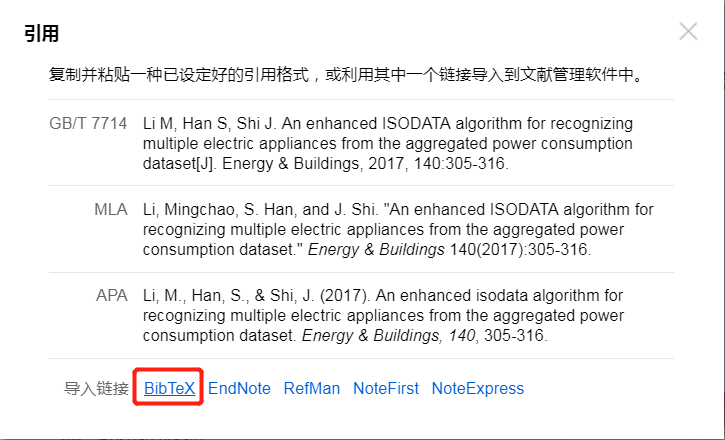
\includegraphics[width=0.6\linewidth]{figures/sample/3-2}
	\caption{导入BibTeX参考文献库步骤二}
	\label{fig:3-2}
\end{figure}

\begin{figure}[htb!]
	\centering
	\begin{subfigure}[b]{.4\textwidth}
		\centering
		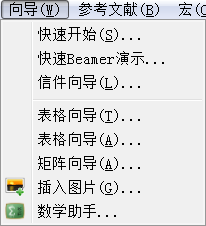
\includegraphics[width=0.7\linewidth]{3-3.png}
		\caption{TeXstudio向导}\label{subfig:3a}
	\end{subfigure}
	\begin{subfigure}[b]{.4\textwidth}
		\centering
		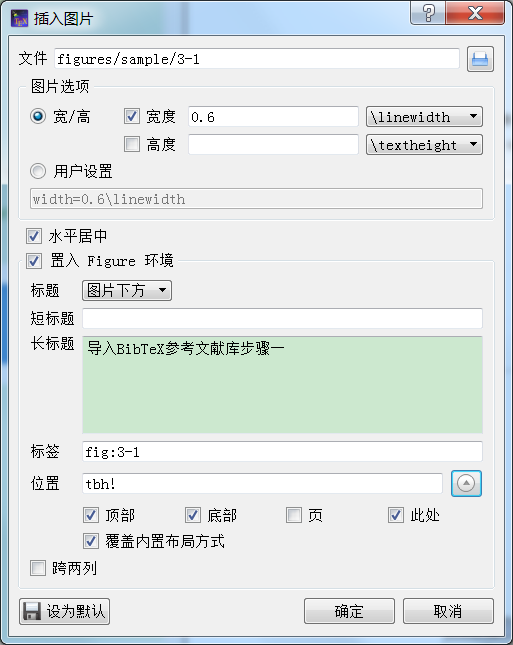
\includegraphics[width=\linewidth]{3-4.png}
		\caption{插入图片}\label{subfig:3b}
	\end{subfigure}
	\caption{使用TeXstudio向导插入图片}\label{fig:3}
\end{figure}
%-----------------------------
\section{意见及问题反馈}

\indent E-mail:wizen\_zhang@163.com\\
\indent GitHub:\href{https://github.com/WizenZhang/NMUThesis/issues}{https://github.com/WizenZhang/NMUThesis/issues}


